\documentclass{whiteboard}
\begin{document}
\begin{frame}[plain,t]
\bbcover{OJ 11573}{Ocean Currents}{Prof. Edson Alves}{Faculdade UnB Gama}

\end{frame}
\begin{frame}[plain,t]
\vspace*{\fill}

\bbenglish{For a boat on a large body of water, strong currents can be dangerous, but with careful planning, they can be harnessed to help the boat reach its destination. Your job is to help in that planning.}

\vspace{0.1in}

\bbenglish{At each location, the current flows in some direction. The captain can choose to either go with the flow of the current, using no energy, or to move one square in any other direction, at the cost of one energy unit. The boat always moves in one of the following eight directions: north, south, east, west, northeast, northwest, southeast, southwest. The boat cannot leave the boundary of the lake.}

\vspace{0.1in}

\bbenglish{You are to help him devise a strategy to reach the destination with the minimum energy consumption.}

\vspace*{\fill}
\end{frame}
\begin{frame}[plain,t]
\vspace*{\fill}

\bbtext{Para um barco, as correntes podem ser perigosas ao se navegar em uma área ampla, mas com um planejamento cuidadoso, estas correntes podem ser usadas para auxiliar o barco a chegar em seu destino. Seu trabalho é auxiliar neste planejamento.}

\vspace{0.1in}

\bbtext{Em cada localidade, as correntes seguem uma certa direção. O capitão pode optar ou por seguir a corrente, sem gastar energia, ou se mover um quadrado em qualquer outra direção, com o custo de uma unidade de energia. O barco sempre se move em uma das seguintes oito direções: norte, sul, leste, oeste, nordeste, noroeste, sudeste, sudoeste. O barco não pode sair da região delimitada pelo lago.}

\vspace{0.1in}

\bbtext{Você deve auxiliá-lo a estabelecer uma estratégia para atingir o seu destino com o menor consumo de energia possível.}

\vspace*{\fill}
\end{frame}
\begin{frame}[plain,t]
\vspace*{\fill}

\bbbold{Input}

\vspace{0.1in}

\bbenglish{The lake is represented as a rectangular grid. The first line of input contains two integers $r$ and $c$, the number of rows and columns in the grid. The grid has no more than $1000$ rows and no more than $1000$ columns. Each of the following $r$ lines contains exactly $c$ characters, each a digit from $0$ to $7$ inclusive.  The character `\texttt{0}' means the current flows north (i.e. up in the grid, in the direction of decreasing row number), `\texttt{1}' means it flows northeast, `\texttt{2}' means east (i.e. in the direction of increasing column number), `\texttt{3}' means southeast, and so on in a clockwise manner:}

\vspace{0.1in}

\begin{center}
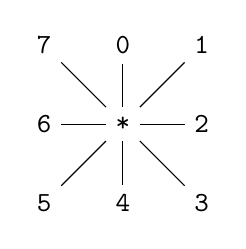
\begin{tikzpicture}[scale=0.5]
\node (A0) at (4, 6) { \tt 0 };
\node (A1) at (6, 6) { \tt 1 };
\node (A2) at (6, 4) { \tt 2 };
\node (A3) at (6, 2) { \tt 3 };
\node (A4) at (4, 2) { \tt 4 };
\node (A5) at (2, 2) { \tt 5 };
\node (A6) at (2, 4) { \tt 6 };
\node (A7) at (2, 6) { \tt 7 };
\node (S) at (4, 4) { \tt * };

\draw (S) to (A0);
\draw (S) to (A1);
\draw (S) to (A2);
\draw (S) to (A3);
\draw (S) to (A4);
\draw (S) to (A5);
\draw (S) to (A6);
\draw (S) to (A7);
\end{tikzpicture}
\end{center}

\vspace*{\fill}
\end{frame}
\begin{frame}[plain,t]
\vspace*{\fill}

\bbbold{Entrada}

\vspace{0.1in}

\bbtext{O lago é representado como uma malha retangular. A primeira linha da entrada contém dois inteiros $r$ e $c$, o número de linhas e de colunas da malha. A malha não tem mais do que $1000$ linhas e não mais do que $1000$ colunas. Cada uma das $r$ linhas seguintes contém exatamente $c$ caracteres, sendo um dos dígitos $0$ a $7$, inclusive.  O caractere `\texttt{0}' significa que a corrente flui para o norte (isto é, para cima na malha, na direção decrescente do número da linha), `\texttt{1}' significa que a corrente flui no sentido nordeste, `\texttt{2}' significa leste (isto é, na direção crescente do número da coluna), `\texttt{3}' significa sudeste, e assim por diante, em sentido horário:}

\vspace{0.1in}

\begin{center}
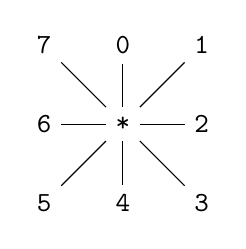
\begin{tikzpicture}[scale=0.5]
\node (A0) at (4, 6) { \tt 0 };
\node (A1) at (6, 6) { \tt 1 };
\node (A2) at (6, 4) { \tt 2 };
\node (A3) at (6, 2) { \tt 3 };
\node (A4) at (4, 2) { \tt 4 };
\node (A5) at (2, 2) { \tt 5 };
\node (A6) at (2, 4) { \tt 6 };
\node (A7) at (2, 6) { \tt 7 };
\node (S) at (4, 4) { \tt * };

\draw (S) to (A0);
\draw (S) to (A1);
\draw (S) to (A2);
\draw (S) to (A3);
\draw (S) to (A4);
\draw (S) to (A5);
\draw (S) to (A6);
\draw (S) to (A7);
\end{tikzpicture}
\end{center}


\vspace*{\fill}
\end{frame}
\begin{frame}[plain,t]
\vspace*{\fill}

\bbenglish{The line after the grid contains a single integer $n$, the number of trips to be made, which is at most $50$. Each of the following $n$ lines describes a trip using four integers $r_s, c_s, r_d, c_d$, giving the row and column of the starting point and the destination of the trip. Rows and columns are numbered starting with $1$.}

\vspace{0.2in}

\bbbold{Output}

\vspace{0.1in}

\bbenglish{For each trip, output a line containing a single integer, the minimum number of energy units needed to get from the starting point to the destination.}

\vspace*{\fill}
\end{frame}
\begin{frame}[plain,t]
\vspace*{\fill}

\bbtext{A linha após a malha contém um único inteiro $n$, o número de viagens que serão feitas, sendo no máximo igual a $50$. Cada uma das $n$ linhas seguintes descrevem uma viagem por meio de quatro inteiros $r_s, c_s, r_d, c_d$, os quais informam a linha e a coluna do ponto de partida e do destino da viagem. Linhas e colunas são numeradas a partir de $1$.}

\vspace{0.2in}

\bbbold{Saída}

\vspace{0.1in}

\bbtext{Para cada viagem imprima uma linha contendo um único inteiro, o número mínimo de unidades de energia gastas para atingir o destino a partir do ponto de partida.}

\vspace*{\fill}
\end{frame}
\begin{frame}[plain,t]
\begin{tikzpicture}
\node[draw,opacity=0] at (0, 0) {x};
\node[draw,opacity=0] at (14, 8) {x};

	\node[anchor=west] (header) at (0, 7.0) { \bbbold{Exemplo de entrada e saída} };

\end{tikzpicture}
\end{frame}
\begin{frame}[plain,t]
\begin{tikzpicture}
\node[draw,opacity=0] at (0, 0) {x};
\node[draw,opacity=0] at (14, 8) {x};

	\node[anchor=west] (header) at (0, 7.0) { \bbbold{Exemplo de entrada e saída} };


	\node[anchor=west] (line1) at (1.0, 6.0) { \bbtext{\texttt{5 5} } };

\end{tikzpicture}
\end{frame}
\begin{frame}[plain,t]
\begin{tikzpicture}
\node[draw,opacity=0] at (0, 0) {x};
\node[draw,opacity=0] at (14, 8) {x};

	\node[anchor=west] (header) at (0, 7.0) { \bbbold{Exemplo de entrada e saída} };


	\node[anchor=west] (line1) at (1.0, 6.0) { \bbtext{\texttt{5 5} } };


	\draw[->,color=BBViolet] (1.25, 5.0) to  (1.25, 5.75);

	\node[] (r) at (1.25, 4.75) { \footnotesize $r$ };

\end{tikzpicture}
\end{frame}
\begin{frame}[plain,t]
\begin{tikzpicture}
\node[draw,opacity=0] at (0, 0) {x};
\node[draw,opacity=0] at (14, 8) {x};

	\node[anchor=west] (header) at (0, 7.0) { \bbbold{Exemplo de entrada e saída} };


	\node[anchor=west] (line1) at (1.0, 6.0) { \bbtext{\texttt{5 5} } };


	\draw[->,color=BBViolet] (1.65, 5.0) to  (1.65, 5.75);

	\node[] (r) at (1.65, 4.75) { \footnotesize $c$ };



\end{tikzpicture}
\end{frame}
\begin{frame}[plain,t]
\begin{tikzpicture}
\node[draw,opacity=0] at (0, 0) {x};
\node[draw,opacity=0] at (14, 8) {x};

	\node[anchor=west] (header) at (0, 7.0) { \bbbold{Exemplo de entrada e saída} };


	\node[anchor=west] (line1) at (1.0, 6.0) { \bbtext{\texttt{5 5} } };







	\draw[thick] (7.0, 1.0) grid  (12.0, 6.0);

\end{tikzpicture}
\end{frame}
\begin{frame}[plain,t]
\begin{tikzpicture}
\node[draw,opacity=0] at (0, 0) {x};
\node[draw,opacity=0] at (14, 8) {x};

	\node[anchor=west] (header) at (0, 7.0) { \bbbold{Exemplo de entrada e saída} };


	\node[anchor=west] (line1) at (1.0, 6.0) { \bbtext{\texttt{5 5} } };







	\draw[thick] (7.0, 1.0) grid  (12.0, 6.0);


	\node[anchor=west] (line2) at (1.0, 5.5) { \bbtext{\texttt{04125} } };

	\node[anchor=west] (line3) at (1.0, 5.0) { \bbtext{\texttt{03355} } };

	\node[anchor=west] (line4) at (1.0, 4.5) { \bbtext{\texttt{64734} } };

	\node[anchor=west] (line5) at (1.0, 4.0) { \bbtext{\texttt{72377} } };

	\node[anchor=west] (line6) at (1.0, 3.5) { \bbtext{\texttt{02062} } };

\end{tikzpicture}
\end{frame}
\begin{frame}[plain,t]
\begin{tikzpicture}
\node[draw,opacity=0] at (0, 0) {x};
\node[draw,opacity=0] at (14, 8) {x};

	\node[anchor=west] (header) at (0, 7.0) { \bbbold{Exemplo de entrada e saída} };


	\node[anchor=west] (line1) at (1.0, 6.0) { \bbtext{\texttt{5 5} } };


	\draw[->,color=BBViolet] (1.65, 2.5) to  (1.65, 3.25);

	\node[] (r) at (1.65, 2.25) { \footnotesize \bbcomment{malha} };




	\draw[thick] (7.0, 1.0) grid  (12.0, 6.0);


	\node[anchor=west] (line2) at (1.0, 5.5) { \bbtext{\texttt{04125} } };

	\node[anchor=west] (line3) at (1.0, 5.0) { \bbtext{\texttt{03355} } };

	\node[anchor=west] (line4) at (1.0, 4.5) { \bbtext{\texttt{64734} } };

	\node[anchor=west] (line5) at (1.0, 4.0) { \bbtext{\texttt{72377} } };

	\node[anchor=west] (line6) at (1.0, 3.5) { \bbtext{\texttt{02062} } };




\end{tikzpicture}
\end{frame}
\begin{frame}[plain,t]
\begin{tikzpicture}
\node[draw,opacity=0] at (0, 0) {x};
\node[draw,opacity=0] at (14, 8) {x};

	\node[anchor=west] (header) at (0, 7.0) { \bbbold{Exemplo de entrada e saída} };


	\node[anchor=west] (line1) at (1.0, 6.0) { \bbtext{\texttt{5 5} } };







	\draw[thick] (7.0, 1.0) grid  (12.0, 6.0);


	\node[anchor=west] (line2) at (1.0, 5.5) { \bbtext{\texttt{04125} } };

	\node[anchor=west] (line3) at (1.0, 5.0) { \bbtext{\texttt{03355} } };

	\node[anchor=west] (line4) at (1.0, 4.5) { \bbtext{\texttt{64734} } };

	\node[anchor=west] (line5) at (1.0, 4.0) { \bbtext{\texttt{72377} } };

	\node[anchor=west] (line6) at (1.0, 3.5) { \bbtext{\texttt{02062} } };






	\node[scale=1.5] (a11) at (7.5, 5.5) { \faArrowUp };

	\node[scale=1.5] (a12) at (8.5, 5.5) { \faArrowDown };

	\node[scale=1.5,rotate=-45] (a13) at (9.5, 5.5) { \faArrowUp };

	\node[scale=1.5] (a14) at (10.5, 5.5) { \faArrowRight };

	\node[scale=1.5,rotate=-45] (a15) at (11.5, 5.5) { \faArrowDown };

	\node[scale=1.5] (a21) at (7.5, 4.5) { \faArrowUp };

	\node[scale=1.5,rotate=45] (a22) at (8.5, 4.5) { \faArrowDown };

	\node[scale=1.5,rotate=45] (a23) at (9.5, 4.5) { \faArrowDown };

	\node[scale=1.5,rotate=-45] (a24) at (10.5, 4.5) { \faArrowDown };

	\node[scale=1.5,rotate=-45] (a25) at (11.5, 4.5) { \faArrowDown };

	\node[scale=1.5] (a31) at (7.5, 3.5) { \faArrowLeft };

	\node[scale=1.5] (a32) at (8.5, 3.5) { \faArrowDown };

	\node[scale=1.5,rotate=-45] (a33) at (9.5, 3.5) { \faArrowLeft };

	\node[scale=1.5,rotate=-45] (a34) at (10.5, 3.5) { \faArrowRight };

	\node[scale=1.5] (a35) at (11.5, 3.5) { \faArrowDown };

	\node[scale=1.5,rotate=45] (a41) at (7.5, 2.5) { \faArrowUp };

	\node[scale=1.5] (a42) at (8.5, 2.5) { \faArrowRight };

	\node[scale=1.5,rotate=-45] (a43) at (9.5, 2.5) { \faArrowRight };

	\node[scale=1.5,rotate=45] (a44) at (10.5, 2.5) { \faArrowUp };

	\node[scale=1.5,rotate=45] (a45) at (11.5, 2.5) { \faArrowUp };

	\node[scale=1.5] (a51) at (7.5, 1.5) { \faArrowUp };

	\node[scale=1.5] (a52) at (8.5, 1.5) { \faArrowRight };

	\node[scale=1.5] (a53) at (9.5, 1.5) { \faArrowUp };

	\node[scale=1.5] (a54) at (10.5, 1.5) { \faArrowLeft };

	\node[scale=1.5] (a55) at (11.5, 1.5) { \faArrowRight };

\end{tikzpicture}
\end{frame}
\begin{frame}[plain,t]
\begin{tikzpicture}
\node[draw,opacity=0] at (0, 0) {x};
\node[draw,opacity=0] at (14, 8) {x};

	\node[anchor=west] (header) at (0, 7.0) { \bbbold{Exemplo de entrada e saída} };


	\node[anchor=west] (line1) at (1.0, 6.0) { \bbtext{\texttt{5 5} } };







	\draw[thick] (7.0, 1.0) grid  (12.0, 6.0);


	\node[anchor=west] (line2) at (1.0, 5.5) { \bbtext{\texttt{04125} } };

	\node[anchor=west] (line3) at (1.0, 5.0) { \bbtext{\texttt{03355} } };

	\node[anchor=west] (line4) at (1.0, 4.5) { \bbtext{\texttt{64734} } };

	\node[anchor=west] (line5) at (1.0, 4.0) { \bbtext{\texttt{72377} } };

	\node[anchor=west] (line6) at (1.0, 3.5) { \bbtext{\texttt{02062} } };






	\node[scale=1.5] (a11) at (7.5, 5.5) { \faArrowUp };

	\node[scale=1.5] (a12) at (8.5, 5.5) { \faArrowDown };

	\node[scale=1.5,rotate=-45] (a13) at (9.5, 5.5) { \faArrowUp };

	\node[scale=1.5] (a14) at (10.5, 5.5) { \faArrowRight };

	\node[scale=1.5,rotate=-45] (a15) at (11.5, 5.5) { \faArrowDown };

	\node[scale=1.5] (a21) at (7.5, 4.5) { \faArrowUp };

	\node[scale=1.5,rotate=45] (a22) at (8.5, 4.5) { \faArrowDown };

	\node[scale=1.5,rotate=45] (a23) at (9.5, 4.5) { \faArrowDown };

	\node[scale=1.5,rotate=-45] (a24) at (10.5, 4.5) { \faArrowDown };

	\node[scale=1.5,rotate=-45] (a25) at (11.5, 4.5) { \faArrowDown };

	\node[scale=1.5] (a31) at (7.5, 3.5) { \faArrowLeft };

	\node[scale=1.5] (a32) at (8.5, 3.5) { \faArrowDown };

	\node[scale=1.5,rotate=-45] (a33) at (9.5, 3.5) { \faArrowLeft };

	\node[scale=1.5,rotate=-45] (a34) at (10.5, 3.5) { \faArrowRight };

	\node[scale=1.5] (a35) at (11.5, 3.5) { \faArrowDown };

	\node[scale=1.5,rotate=45] (a41) at (7.5, 2.5) { \faArrowUp };

	\node[scale=1.5] (a42) at (8.5, 2.5) { \faArrowRight };

	\node[scale=1.5,rotate=-45] (a43) at (9.5, 2.5) { \faArrowRight };

	\node[scale=1.5,rotate=45] (a44) at (10.5, 2.5) { \faArrowUp };

	\node[scale=1.5,rotate=45] (a45) at (11.5, 2.5) { \faArrowUp };

	\node[scale=1.5] (a51) at (7.5, 1.5) { \faArrowUp };

	\node[scale=1.5] (a52) at (8.5, 1.5) { \faArrowRight };

	\node[scale=1.5] (a53) at (9.5, 1.5) { \faArrowUp };

	\node[scale=1.5] (a54) at (10.5, 1.5) { \faArrowLeft };

	\node[scale=1.5] (a55) at (11.5, 1.5) { \faArrowRight };


	\node[anchor=west] (line7) at (1.0, 3.0) { \bbtext{\texttt{3} } };

\end{tikzpicture}
\end{frame}
\begin{frame}[plain,t]
\begin{tikzpicture}
\node[draw,opacity=0] at (0, 0) {x};
\node[draw,opacity=0] at (14, 8) {x};

	\node[anchor=west] (header) at (0, 7.0) { \bbbold{Exemplo de entrada e saída} };


	\node[anchor=west] (line1) at (1.0, 6.0) { \bbtext{\texttt{5 5} } };


	\draw[->,color=BBViolet] (1.25, 2.0) to  (1.25, 2.75);

	\node[] (r) at (1.25, 1.75) { \footnotesize \bbcomment{\# de viagens} };




	\draw[thick] (7.0, 1.0) grid  (12.0, 6.0);


	\node[anchor=west] (line2) at (1.0, 5.5) { \bbtext{\texttt{04125} } };

	\node[anchor=west] (line3) at (1.0, 5.0) { \bbtext{\texttt{03355} } };

	\node[anchor=west] (line4) at (1.0, 4.5) { \bbtext{\texttt{64734} } };

	\node[anchor=west] (line5) at (1.0, 4.0) { \bbtext{\texttt{72377} } };

	\node[anchor=west] (line6) at (1.0, 3.5) { \bbtext{\texttt{02062} } };






	\node[scale=1.5] (a11) at (7.5, 5.5) { \faArrowUp };

	\node[scale=1.5] (a12) at (8.5, 5.5) { \faArrowDown };

	\node[scale=1.5,rotate=-45] (a13) at (9.5, 5.5) { \faArrowUp };

	\node[scale=1.5] (a14) at (10.5, 5.5) { \faArrowRight };

	\node[scale=1.5,rotate=-45] (a15) at (11.5, 5.5) { \faArrowDown };

	\node[scale=1.5] (a21) at (7.5, 4.5) { \faArrowUp };

	\node[scale=1.5,rotate=45] (a22) at (8.5, 4.5) { \faArrowDown };

	\node[scale=1.5,rotate=45] (a23) at (9.5, 4.5) { \faArrowDown };

	\node[scale=1.5,rotate=-45] (a24) at (10.5, 4.5) { \faArrowDown };

	\node[scale=1.5,rotate=-45] (a25) at (11.5, 4.5) { \faArrowDown };

	\node[scale=1.5] (a31) at (7.5, 3.5) { \faArrowLeft };

	\node[scale=1.5] (a32) at (8.5, 3.5) { \faArrowDown };

	\node[scale=1.5,rotate=-45] (a33) at (9.5, 3.5) { \faArrowLeft };

	\node[scale=1.5,rotate=-45] (a34) at (10.5, 3.5) { \faArrowRight };

	\node[scale=1.5] (a35) at (11.5, 3.5) { \faArrowDown };

	\node[scale=1.5,rotate=45] (a41) at (7.5, 2.5) { \faArrowUp };

	\node[scale=1.5] (a42) at (8.5, 2.5) { \faArrowRight };

	\node[scale=1.5,rotate=-45] (a43) at (9.5, 2.5) { \faArrowRight };

	\node[scale=1.5,rotate=45] (a44) at (10.5, 2.5) { \faArrowUp };

	\node[scale=1.5,rotate=45] (a45) at (11.5, 2.5) { \faArrowUp };

	\node[scale=1.5] (a51) at (7.5, 1.5) { \faArrowUp };

	\node[scale=1.5] (a52) at (8.5, 1.5) { \faArrowRight };

	\node[scale=1.5] (a53) at (9.5, 1.5) { \faArrowUp };

	\node[scale=1.5] (a54) at (10.5, 1.5) { \faArrowLeft };

	\node[scale=1.5] (a55) at (11.5, 1.5) { \faArrowRight };


	\node[anchor=west] (line7) at (1.0, 3.0) { \bbtext{\texttt{3} } };




\end{tikzpicture}
\end{frame}
\begin{frame}[plain,t]
\begin{tikzpicture}
\node[draw,opacity=0] at (0, 0) {x};
\node[draw,opacity=0] at (14, 8) {x};

	\node[anchor=west] (header) at (0, 7.0) { \bbbold{Exemplo de entrada e saída} };


	\node[anchor=west] (line1) at (1.0, 6.0) { \bbtext{\texttt{5 5} } };







	\draw[thick] (7.0, 1.0) grid  (12.0, 6.0);


	\node[anchor=west] (line2) at (1.0, 5.5) { \bbtext{\texttt{04125} } };

	\node[anchor=west] (line3) at (1.0, 5.0) { \bbtext{\texttt{03355} } };

	\node[anchor=west] (line4) at (1.0, 4.5) { \bbtext{\texttt{64734} } };

	\node[anchor=west] (line5) at (1.0, 4.0) { \bbtext{\texttt{72377} } };

	\node[anchor=west] (line6) at (1.0, 3.5) { \bbtext{\texttt{02062} } };






	\node[scale=1.5] (a11) at (7.5, 5.5) { \faArrowUp };

	\node[scale=1.5] (a12) at (8.5, 5.5) { \faArrowDown };

	\node[scale=1.5,rotate=-45] (a13) at (9.5, 5.5) { \faArrowUp };

	\node[scale=1.5] (a14) at (10.5, 5.5) { \faArrowRight };

	\node[scale=1.5,rotate=-45] (a15) at (11.5, 5.5) { \faArrowDown };

	\node[scale=1.5] (a21) at (7.5, 4.5) { \faArrowUp };

	\node[scale=1.5,rotate=45] (a22) at (8.5, 4.5) { \faArrowDown };

	\node[scale=1.5,rotate=45] (a23) at (9.5, 4.5) { \faArrowDown };

	\node[scale=1.5,rotate=-45] (a24) at (10.5, 4.5) { \faArrowDown };

	\node[scale=1.5,rotate=-45] (a25) at (11.5, 4.5) { \faArrowDown };

	\node[scale=1.5] (a31) at (7.5, 3.5) { \faArrowLeft };

	\node[scale=1.5] (a32) at (8.5, 3.5) { \faArrowDown };

	\node[scale=1.5,rotate=-45] (a33) at (9.5, 3.5) { \faArrowLeft };

	\node[scale=1.5,rotate=-45] (a34) at (10.5, 3.5) { \faArrowRight };

	\node[scale=1.5] (a35) at (11.5, 3.5) { \faArrowDown };

	\node[scale=1.5,rotate=45] (a41) at (7.5, 2.5) { \faArrowUp };

	\node[scale=1.5] (a42) at (8.5, 2.5) { \faArrowRight };

	\node[scale=1.5,rotate=-45] (a43) at (9.5, 2.5) { \faArrowRight };

	\node[scale=1.5,rotate=45] (a44) at (10.5, 2.5) { \faArrowUp };

	\node[scale=1.5,rotate=45] (a45) at (11.5, 2.5) { \faArrowUp };

	\node[scale=1.5] (a51) at (7.5, 1.5) { \faArrowUp };

	\node[scale=1.5] (a52) at (8.5, 1.5) { \faArrowRight };

	\node[scale=1.5] (a53) at (9.5, 1.5) { \faArrowUp };

	\node[scale=1.5] (a54) at (10.5, 1.5) { \faArrowLeft };

	\node[scale=1.5] (a55) at (11.5, 1.5) { \faArrowRight };


	\node[anchor=west] (line7) at (1.0, 3.0) { \bbtext{\texttt{3} } };






	\node[anchor=west] (line8) at (1.0, 2.5) { \bbtext{\texttt{4 2 4 2} } };

\end{tikzpicture}
\end{frame}
\begin{frame}[plain,t]
\begin{tikzpicture}
\node[draw,opacity=0] at (0, 0) {x};
\node[draw,opacity=0] at (14, 8) {x};

	\node[anchor=west] (header) at (0, 7.0) { \bbbold{Exemplo de entrada e saída} };


	\node[anchor=west] (line1) at (1.0, 6.0) { \bbtext{\texttt{5 5} } };


	\draw[->,color=BBViolet] (1.25, 1.5) to  (1.25, 2.25);

	\node[] (r) at (1.25, 1.25) { \footnotesize $r_s$ };




	\draw[thick] (7.0, 1.0) grid  (12.0, 6.0);


	\node[anchor=west] (line2) at (1.0, 5.5) { \bbtext{\texttt{04125} } };

	\node[anchor=west] (line3) at (1.0, 5.0) { \bbtext{\texttt{03355} } };

	\node[anchor=west] (line4) at (1.0, 4.5) { \bbtext{\texttt{64734} } };

	\node[anchor=west] (line5) at (1.0, 4.0) { \bbtext{\texttt{72377} } };

	\node[anchor=west] (line6) at (1.0, 3.5) { \bbtext{\texttt{02062} } };






	\node[scale=1.5] (a11) at (7.5, 5.5) { \faArrowUp };

	\node[scale=1.5] (a12) at (8.5, 5.5) { \faArrowDown };

	\node[scale=1.5,rotate=-45] (a13) at (9.5, 5.5) { \faArrowUp };

	\node[scale=1.5] (a14) at (10.5, 5.5) { \faArrowRight };

	\node[scale=1.5,rotate=-45] (a15) at (11.5, 5.5) { \faArrowDown };

	\node[scale=1.5] (a21) at (7.5, 4.5) { \faArrowUp };

	\node[scale=1.5,rotate=45] (a22) at (8.5, 4.5) { \faArrowDown };

	\node[scale=1.5,rotate=45] (a23) at (9.5, 4.5) { \faArrowDown };

	\node[scale=1.5,rotate=-45] (a24) at (10.5, 4.5) { \faArrowDown };

	\node[scale=1.5,rotate=-45] (a25) at (11.5, 4.5) { \faArrowDown };

	\node[scale=1.5] (a31) at (7.5, 3.5) { \faArrowLeft };

	\node[scale=1.5] (a32) at (8.5, 3.5) { \faArrowDown };

	\node[scale=1.5,rotate=-45] (a33) at (9.5, 3.5) { \faArrowLeft };

	\node[scale=1.5,rotate=-45] (a34) at (10.5, 3.5) { \faArrowRight };

	\node[scale=1.5] (a35) at (11.5, 3.5) { \faArrowDown };

	\node[scale=1.5,rotate=45] (a41) at (7.5, 2.5) { \faArrowUp };

	\node[scale=1.5] (a42) at (8.5, 2.5) { \faArrowRight };

	\node[scale=1.5,rotate=-45] (a43) at (9.5, 2.5) { \faArrowRight };

	\node[scale=1.5,rotate=45] (a44) at (10.5, 2.5) { \faArrowUp };

	\node[scale=1.5,rotate=45] (a45) at (11.5, 2.5) { \faArrowUp };

	\node[scale=1.5] (a51) at (7.5, 1.5) { \faArrowUp };

	\node[scale=1.5] (a52) at (8.5, 1.5) { \faArrowRight };

	\node[scale=1.5] (a53) at (9.5, 1.5) { \faArrowUp };

	\node[scale=1.5] (a54) at (10.5, 1.5) { \faArrowLeft };

	\node[scale=1.5] (a55) at (11.5, 1.5) { \faArrowRight };


	\node[anchor=west] (line7) at (1.0, 3.0) { \bbtext{\texttt{3} } };






	\node[anchor=west] (line8) at (1.0, 2.5) { \bbtext{\texttt{4 2 4 2} } };




\end{tikzpicture}
\end{frame}
\begin{frame}[plain,t]
\begin{tikzpicture}
\node[draw,opacity=0] at (0, 0) {x};
\node[draw,opacity=0] at (14, 8) {x};

	\node[anchor=west] (header) at (0, 7.0) { \bbbold{Exemplo de entrada e saída} };


	\node[anchor=west] (line1) at (1.0, 6.0) { \bbtext{\texttt{5 5} } };


	\draw[->,color=BBViolet] (1.65, 1.5) to  (1.65, 2.25);

	\node[] (r) at (1.65, 1.25) { \footnotesize $c_s$ };




	\draw[thick] (7.0, 1.0) grid  (12.0, 6.0);


	\node[anchor=west] (line2) at (1.0, 5.5) { \bbtext{\texttt{04125} } };

	\node[anchor=west] (line3) at (1.0, 5.0) { \bbtext{\texttt{03355} } };

	\node[anchor=west] (line4) at (1.0, 4.5) { \bbtext{\texttt{64734} } };

	\node[anchor=west] (line5) at (1.0, 4.0) { \bbtext{\texttt{72377} } };

	\node[anchor=west] (line6) at (1.0, 3.5) { \bbtext{\texttt{02062} } };






	\node[scale=1.5] (a11) at (7.5, 5.5) { \faArrowUp };

	\node[scale=1.5] (a12) at (8.5, 5.5) { \faArrowDown };

	\node[scale=1.5,rotate=-45] (a13) at (9.5, 5.5) { \faArrowUp };

	\node[scale=1.5] (a14) at (10.5, 5.5) { \faArrowRight };

	\node[scale=1.5,rotate=-45] (a15) at (11.5, 5.5) { \faArrowDown };

	\node[scale=1.5] (a21) at (7.5, 4.5) { \faArrowUp };

	\node[scale=1.5,rotate=45] (a22) at (8.5, 4.5) { \faArrowDown };

	\node[scale=1.5,rotate=45] (a23) at (9.5, 4.5) { \faArrowDown };

	\node[scale=1.5,rotate=-45] (a24) at (10.5, 4.5) { \faArrowDown };

	\node[scale=1.5,rotate=-45] (a25) at (11.5, 4.5) { \faArrowDown };

	\node[scale=1.5] (a31) at (7.5, 3.5) { \faArrowLeft };

	\node[scale=1.5] (a32) at (8.5, 3.5) { \faArrowDown };

	\node[scale=1.5,rotate=-45] (a33) at (9.5, 3.5) { \faArrowLeft };

	\node[scale=1.5,rotate=-45] (a34) at (10.5, 3.5) { \faArrowRight };

	\node[scale=1.5] (a35) at (11.5, 3.5) { \faArrowDown };

	\node[scale=1.5,rotate=45] (a41) at (7.5, 2.5) { \faArrowUp };

	\node[scale=1.5] (a42) at (8.5, 2.5) { \faArrowRight };

	\node[scale=1.5,rotate=-45] (a43) at (9.5, 2.5) { \faArrowRight };

	\node[scale=1.5,rotate=45] (a44) at (10.5, 2.5) { \faArrowUp };

	\node[scale=1.5,rotate=45] (a45) at (11.5, 2.5) { \faArrowUp };

	\node[scale=1.5] (a51) at (7.5, 1.5) { \faArrowUp };

	\node[scale=1.5] (a52) at (8.5, 1.5) { \faArrowRight };

	\node[scale=1.5] (a53) at (9.5, 1.5) { \faArrowUp };

	\node[scale=1.5] (a54) at (10.5, 1.5) { \faArrowLeft };

	\node[scale=1.5] (a55) at (11.5, 1.5) { \faArrowRight };


	\node[anchor=west] (line7) at (1.0, 3.0) { \bbtext{\texttt{3} } };






	\node[anchor=west] (line8) at (1.0, 2.5) { \bbtext{\texttt{4 2 4 2} } };







\end{tikzpicture}
\end{frame}
\begin{frame}[plain,t]
\begin{tikzpicture}
\node[draw,opacity=0] at (0, 0) {x};
\node[draw,opacity=0] at (14, 8) {x};

	\node[anchor=west] (header) at (0, 7.0) { \bbbold{Exemplo de entrada e saída} };


	\node[anchor=west] (line1) at (1.0, 6.0) { \bbtext{\texttt{5 5} } };


	\draw[->,color=BBViolet] (2.05, 1.5) to  (2.05, 2.25);

	\node[] (r) at (2.05, 1.25) { \footnotesize $r_d$ };




	\draw[thick] (7.0, 1.0) grid  (12.0, 6.0);


	\node[anchor=west] (line2) at (1.0, 5.5) { \bbtext{\texttt{04125} } };

	\node[anchor=west] (line3) at (1.0, 5.0) { \bbtext{\texttt{03355} } };

	\node[anchor=west] (line4) at (1.0, 4.5) { \bbtext{\texttt{64734} } };

	\node[anchor=west] (line5) at (1.0, 4.0) { \bbtext{\texttt{72377} } };

	\node[anchor=west] (line6) at (1.0, 3.5) { \bbtext{\texttt{02062} } };






	\node[scale=1.5] (a11) at (7.5, 5.5) { \faArrowUp };

	\node[scale=1.5] (a12) at (8.5, 5.5) { \faArrowDown };

	\node[scale=1.5,rotate=-45] (a13) at (9.5, 5.5) { \faArrowUp };

	\node[scale=1.5] (a14) at (10.5, 5.5) { \faArrowRight };

	\node[scale=1.5,rotate=-45] (a15) at (11.5, 5.5) { \faArrowDown };

	\node[scale=1.5] (a21) at (7.5, 4.5) { \faArrowUp };

	\node[scale=1.5,rotate=45] (a22) at (8.5, 4.5) { \faArrowDown };

	\node[scale=1.5,rotate=45] (a23) at (9.5, 4.5) { \faArrowDown };

	\node[scale=1.5,rotate=-45] (a24) at (10.5, 4.5) { \faArrowDown };

	\node[scale=1.5,rotate=-45] (a25) at (11.5, 4.5) { \faArrowDown };

	\node[scale=1.5] (a31) at (7.5, 3.5) { \faArrowLeft };

	\node[scale=1.5] (a32) at (8.5, 3.5) { \faArrowDown };

	\node[scale=1.5,rotate=-45] (a33) at (9.5, 3.5) { \faArrowLeft };

	\node[scale=1.5,rotate=-45] (a34) at (10.5, 3.5) { \faArrowRight };

	\node[scale=1.5] (a35) at (11.5, 3.5) { \faArrowDown };

	\node[scale=1.5,rotate=45] (a41) at (7.5, 2.5) { \faArrowUp };

	\node[scale=1.5] (a42) at (8.5, 2.5) { \faArrowRight };

	\node[scale=1.5,rotate=-45] (a43) at (9.5, 2.5) { \faArrowRight };

	\node[scale=1.5,rotate=45] (a44) at (10.5, 2.5) { \faArrowUp };

	\node[scale=1.5,rotate=45] (a45) at (11.5, 2.5) { \faArrowUp };

	\node[scale=1.5] (a51) at (7.5, 1.5) { \faArrowUp };

	\node[scale=1.5] (a52) at (8.5, 1.5) { \faArrowRight };

	\node[scale=1.5] (a53) at (9.5, 1.5) { \faArrowUp };

	\node[scale=1.5] (a54) at (10.5, 1.5) { \faArrowLeft };

	\node[scale=1.5] (a55) at (11.5, 1.5) { \faArrowRight };


	\node[anchor=west] (line7) at (1.0, 3.0) { \bbtext{\texttt{3} } };






	\node[anchor=west] (line8) at (1.0, 2.5) { \bbtext{\texttt{4 2 4 2} } };










\end{tikzpicture}
\end{frame}
\begin{frame}[plain,t]
\begin{tikzpicture}
\node[draw,opacity=0] at (0, 0) {x};
\node[draw,opacity=0] at (14, 8) {x};

	\node[anchor=west] (header) at (0, 7.0) { \bbbold{Exemplo de entrada e saída} };


	\node[anchor=west] (line1) at (1.0, 6.0) { \bbtext{\texttt{5 5} } };


	\draw[->,color=BBViolet] (2.45, 1.5) to  (2.45, 2.25);

	\node[] (r) at (2.45, 1.25) { \footnotesize $r_s$ };




	\draw[thick] (7.0, 1.0) grid  (12.0, 6.0);


	\node[anchor=west] (line2) at (1.0, 5.5) { \bbtext{\texttt{04125} } };

	\node[anchor=west] (line3) at (1.0, 5.0) { \bbtext{\texttt{03355} } };

	\node[anchor=west] (line4) at (1.0, 4.5) { \bbtext{\texttt{64734} } };

	\node[anchor=west] (line5) at (1.0, 4.0) { \bbtext{\texttt{72377} } };

	\node[anchor=west] (line6) at (1.0, 3.5) { \bbtext{\texttt{02062} } };






	\node[scale=1.5] (a11) at (7.5, 5.5) { \faArrowUp };

	\node[scale=1.5] (a12) at (8.5, 5.5) { \faArrowDown };

	\node[scale=1.5,rotate=-45] (a13) at (9.5, 5.5) { \faArrowUp };

	\node[scale=1.5] (a14) at (10.5, 5.5) { \faArrowRight };

	\node[scale=1.5,rotate=-45] (a15) at (11.5, 5.5) { \faArrowDown };

	\node[scale=1.5] (a21) at (7.5, 4.5) { \faArrowUp };

	\node[scale=1.5,rotate=45] (a22) at (8.5, 4.5) { \faArrowDown };

	\node[scale=1.5,rotate=45] (a23) at (9.5, 4.5) { \faArrowDown };

	\node[scale=1.5,rotate=-45] (a24) at (10.5, 4.5) { \faArrowDown };

	\node[scale=1.5,rotate=-45] (a25) at (11.5, 4.5) { \faArrowDown };

	\node[scale=1.5] (a31) at (7.5, 3.5) { \faArrowLeft };

	\node[scale=1.5] (a32) at (8.5, 3.5) { \faArrowDown };

	\node[scale=1.5,rotate=-45] (a33) at (9.5, 3.5) { \faArrowLeft };

	\node[scale=1.5,rotate=-45] (a34) at (10.5, 3.5) { \faArrowRight };

	\node[scale=1.5] (a35) at (11.5, 3.5) { \faArrowDown };

	\node[scale=1.5,rotate=45] (a41) at (7.5, 2.5) { \faArrowUp };

	\node[scale=1.5] (a42) at (8.5, 2.5) { \faArrowRight };

	\node[scale=1.5,rotate=-45] (a43) at (9.5, 2.5) { \faArrowRight };

	\node[scale=1.5,rotate=45] (a44) at (10.5, 2.5) { \faArrowUp };

	\node[scale=1.5,rotate=45] (a45) at (11.5, 2.5) { \faArrowUp };

	\node[scale=1.5] (a51) at (7.5, 1.5) { \faArrowUp };

	\node[scale=1.5] (a52) at (8.5, 1.5) { \faArrowRight };

	\node[scale=1.5] (a53) at (9.5, 1.5) { \faArrowUp };

	\node[scale=1.5] (a54) at (10.5, 1.5) { \faArrowLeft };

	\node[scale=1.5] (a55) at (11.5, 1.5) { \faArrowRight };


	\node[anchor=west] (line7) at (1.0, 3.0) { \bbtext{\texttt{3} } };






	\node[anchor=west] (line8) at (1.0, 2.5) { \bbtext{\texttt{4 2 4 2} } };













\end{tikzpicture}
\end{frame}
\begin{frame}[plain,t]
\begin{tikzpicture}
\node[draw,opacity=0] at (0, 0) {x};
\node[draw,opacity=0] at (14, 8) {x};

	\node[anchor=west] (header) at (0, 7.0) { \bbbold{Exemplo de entrada e saída} };


	\node[anchor=west] (line1) at (1.0, 6.0) { \bbtext{\texttt{5 5} } };


	\draw[->,color=BBBlack,very thick,-latex] (3.0, 2.5) to  (4.0, 2.5);

	\node[anchor=west] (r) at (4.0, 2.5) { \bbinfo{0} };




	\draw[thick] (7.0, 1.0) grid  (12.0, 6.0);


	\node[anchor=west] (line2) at (1.0, 5.5) { \bbtext{\texttt{04125} } };

	\node[anchor=west] (line3) at (1.0, 5.0) { \bbtext{\texttt{03355} } };

	\node[anchor=west] (line4) at (1.0, 4.5) { \bbtext{\texttt{64734} } };

	\node[anchor=west] (line5) at (1.0, 4.0) { \bbtext{\texttt{72377} } };

	\node[anchor=west] (line6) at (1.0, 3.5) { \bbtext{\texttt{02062} } };






	\node[scale=1.5] (a11) at (7.5, 5.5) { \faArrowUp };

	\node[scale=1.5] (a12) at (8.5, 5.5) { \faArrowDown };

	\node[scale=1.5,rotate=-45] (a13) at (9.5, 5.5) { \faArrowUp };

	\node[scale=1.5] (a14) at (10.5, 5.5) { \faArrowRight };

	\node[scale=1.5,rotate=-45] (a15) at (11.5, 5.5) { \faArrowDown };

	\node[scale=1.5] (a21) at (7.5, 4.5) { \faArrowUp };

	\node[scale=1.5,rotate=45] (a22) at (8.5, 4.5) { \faArrowDown };

	\node[scale=1.5,rotate=45] (a23) at (9.5, 4.5) { \faArrowDown };

	\node[scale=1.5,rotate=-45] (a24) at (10.5, 4.5) { \faArrowDown };

	\node[scale=1.5,rotate=-45] (a25) at (11.5, 4.5) { \faArrowDown };

	\node[scale=1.5] (a31) at (7.5, 3.5) { \faArrowLeft };

	\node[scale=1.5] (a32) at (8.5, 3.5) { \faArrowDown };

	\node[scale=1.5,rotate=-45] (a33) at (9.5, 3.5) { \faArrowLeft };

	\node[scale=1.5,rotate=-45] (a34) at (10.5, 3.5) { \faArrowRight };

	\node[scale=1.5] (a35) at (11.5, 3.5) { \faArrowDown };

	\node[scale=1.5,rotate=45] (a41) at (7.5, 2.5) { \faArrowUp };

	\node[scale=1.5] (a42) at (8.5, 2.5) { \textcolor{BBGreen}{\faArrowRight} };

	\node[scale=1.5,rotate=-45] (a43) at (9.5, 2.5) { \faArrowRight };

	\node[scale=1.5,rotate=45] (a44) at (10.5, 2.5) { \faArrowUp };

	\node[scale=1.5,rotate=45] (a45) at (11.5, 2.5) { \faArrowUp };

	\node[scale=1.5] (a51) at (7.5, 1.5) { \faArrowUp };

	\node[scale=1.5] (a52) at (8.5, 1.5) { \faArrowRight };

	\node[scale=1.5] (a53) at (9.5, 1.5) { \faArrowUp };

	\node[scale=1.5] (a54) at (10.5, 1.5) { \faArrowLeft };

	\node[scale=1.5] (a55) at (11.5, 1.5) { \faArrowRight };


	\node[anchor=west] (line7) at (1.0, 3.0) { \bbtext{\texttt{3} } };






	\node[anchor=west] (line8) at (1.0, 2.5) { \bbtext{\texttt{4 2 4 2} } };
















\end{tikzpicture}
\end{frame}
\begin{frame}[plain,t]
\begin{tikzpicture}
\node[draw,opacity=0] at (0, 0) {x};
\node[draw,opacity=0] at (14, 8) {x};

	\node[anchor=west] (header) at (0, 7.0) { \bbbold{Exemplo de entrada e saída} };


	\node[anchor=west] (line1) at (1.0, 6.0) { \bbtext{\texttt{5 5} } };







	\draw[thick] (7.0, 1.0) grid  (12.0, 6.0);


	\node[anchor=west] (line2) at (1.0, 5.5) { \bbtext{\texttt{04125} } };

	\node[anchor=west] (line3) at (1.0, 5.0) { \bbtext{\texttt{03355} } };

	\node[anchor=west] (line4) at (1.0, 4.5) { \bbtext{\texttt{64734} } };

	\node[anchor=west] (line5) at (1.0, 4.0) { \bbtext{\texttt{72377} } };

	\node[anchor=west] (line6) at (1.0, 3.5) { \bbtext{\texttt{02062} } };






	\node[scale=1.5] (a11) at (7.5, 5.5) { \faArrowUp };

	\node[scale=1.5] (a12) at (8.5, 5.5) { \faArrowDown };

	\node[scale=1.5,rotate=-45] (a13) at (9.5, 5.5) { \faArrowUp };

	\node[scale=1.5] (a14) at (10.5, 5.5) { \faArrowRight };

	\node[scale=1.5,rotate=-45] (a15) at (11.5, 5.5) { \faArrowDown };

	\node[scale=1.5] (a21) at (7.5, 4.5) { \faArrowUp };

	\node[scale=1.5,rotate=45] (a22) at (8.5, 4.5) { \faArrowDown };

	\node[scale=1.5,rotate=45] (a23) at (9.5, 4.5) { \faArrowDown };

	\node[scale=1.5,rotate=-45] (a24) at (10.5, 4.5) { \faArrowDown };

	\node[scale=1.5,rotate=-45] (a25) at (11.5, 4.5) { \faArrowDown };

	\node[scale=1.5] (a31) at (7.5, 3.5) { \faArrowLeft };

	\node[scale=1.5] (a32) at (8.5, 3.5) { \faArrowDown };

	\node[scale=1.5,rotate=-45] (a33) at (9.5, 3.5) { \faArrowLeft };

	\node[scale=1.5,rotate=-45] (a34) at (10.5, 3.5) { \faArrowRight };

	\node[scale=1.5] (a35) at (11.5, 3.5) { \faArrowDown };

	\node[scale=1.5,rotate=45] (a41) at (7.5, 2.5) { \faArrowUp };

	\node[scale=1.5] (a42) at (8.5, 2.5) { \textcolor{BBBlack}{\faArrowRight} };

	\node[scale=1.5,rotate=-45] (a43) at (9.5, 2.5) { \faArrowRight };

	\node[scale=1.5,rotate=45] (a44) at (10.5, 2.5) { \faArrowUp };

	\node[scale=1.5,rotate=45] (a45) at (11.5, 2.5) { \faArrowUp };

	\node[scale=1.5] (a51) at (7.5, 1.5) { \faArrowUp };

	\node[scale=1.5] (a52) at (8.5, 1.5) { \faArrowRight };

	\node[scale=1.5] (a53) at (9.5, 1.5) { \faArrowUp };

	\node[scale=1.5] (a54) at (10.5, 1.5) { \faArrowLeft };

	\node[scale=1.5] (a55) at (11.5, 1.5) { \faArrowRight };


	\node[anchor=west] (line7) at (1.0, 3.0) { \bbtext{\texttt{3} } };






	\node[anchor=west] (line8) at (1.0, 2.5) { \bbtext{\texttt{4 2 4 2} } };


















	\node[anchor=west] (line9) at (1.0, 2.0) { \bbtext{\texttt{4 5 1 4} } };

\end{tikzpicture}
\end{frame}
\begin{frame}[plain,t]
\begin{tikzpicture}
\node[draw,opacity=0] at (0, 0) {x};
\node[draw,opacity=0] at (14, 8) {x};

	\node[anchor=west] (header) at (0, 7.0) { \bbbold{Exemplo de entrada e saída} };


	\node[anchor=west] (line1) at (1.0, 6.0) { \bbtext{\texttt{5 5} } };


	\draw[->,color=BBBlack,very thick,-latex] (3.0, 2.0) to  (4.0, 2.0);

	\node[anchor=west] (r) at (4.0, 2.0) { \bbinfo{2} };




	\draw[thick] (7.0, 1.0) grid  (12.0, 6.0);


	\node[anchor=west] (line2) at (1.0, 5.5) { \bbtext{\texttt{04125} } };

	\node[anchor=west] (line3) at (1.0, 5.0) { \bbtext{\texttt{03355} } };

	\node[anchor=west] (line4) at (1.0, 4.5) { \bbtext{\texttt{64734} } };

	\node[anchor=west] (line5) at (1.0, 4.0) { \bbtext{\texttt{72377} } };

	\node[anchor=west] (line6) at (1.0, 3.5) { \bbtext{\texttt{02062} } };






	\node[scale=1.5] (a11) at (7.5, 5.5) { \faArrowUp };

	\node[scale=1.5] (a12) at (8.5, 5.5) { \faArrowDown };

	\node[scale=1.5,rotate=-45] (a13) at (9.5, 5.5) { \faArrowUp };

	\node[scale=1.5] (a14) at (10.5, 5.5) { \textcolor{BBGreen}{\faArrowRight} };

	\node[scale=1.5,rotate=-45] (a15) at (11.5, 5.5) { \faArrowDown };

	\node[scale=1.5] (a21) at (7.5, 4.5) { \faArrowUp };

	\node[scale=1.5,rotate=45] (a22) at (8.5, 4.5) { \faArrowDown };

	\node[scale=1.5,rotate=45] (a23) at (9.5, 4.5) { \faArrowDown };

	\node[scale=1.5,rotate=-45] (a24) at (10.5, 4.5) { \textcolor{BBRed}{\faArrowDown} };

	\node[scale=1.5,rotate=-45] (a25) at (11.5, 4.5) { \faArrowDown };

	\node[scale=1.5] (a31) at (7.5, 3.5) { \faArrowLeft };

	\node[scale=1.5] (a32) at (8.5, 3.5) { \faArrowDown };

	\node[scale=1.5,rotate=-45] (a33) at (9.5, 3.5) { \faArrowLeft };

	\node[scale=1.5,rotate=-45] (a34) at (10.5, 3.5) { \textcolor{BBRed}{\faArrowRight} };

	\node[scale=1.5] (a35) at (11.5, 3.5) { \faArrowDown };

	\node[scale=1.5,rotate=45] (a41) at (7.5, 2.5) { \faArrowUp };

	\node[scale=1.5] (a42) at (8.5, 2.5) { \textcolor{BBBlack}{\faArrowRight} };

	\node[scale=1.5,rotate=-45] (a43) at (9.5, 2.5) { \faArrowRight };

	\node[scale=1.5,rotate=45] (a44) at (10.5, 2.5) { \faArrowUp };

	\node[scale=1.5,rotate=45] (a45) at (11.5, 2.5) { \textcolor{BBCyan}{\faArrowUp} };

	\node[scale=1.5] (a51) at (7.5, 1.5) { \faArrowUp };

	\node[scale=1.5] (a52) at (8.5, 1.5) { \faArrowRight };

	\node[scale=1.5] (a53) at (9.5, 1.5) { \faArrowUp };

	\node[scale=1.5] (a54) at (10.5, 1.5) { \faArrowLeft };

	\node[scale=1.5] (a55) at (11.5, 1.5) { \faArrowRight };


	\node[anchor=west] (line7) at (1.0, 3.0) { \bbtext{\texttt{3} } };






	\node[anchor=west] (line8) at (1.0, 2.5) { \bbtext{\texttt{4 2 4 2} } };


















	\node[anchor=west] (line9) at (1.0, 2.0) { \bbtext{\texttt{4 5 1 4} } };





\end{tikzpicture}
\end{frame}
\begin{frame}[plain,t]
\begin{tikzpicture}
\node[draw,opacity=0] at (0, 0) {x};
\node[draw,opacity=0] at (14, 8) {x};

	\node[anchor=west] (header) at (0, 7.0) { \bbbold{Exemplo de entrada e saída} };


	\node[anchor=west] (line1) at (1.0, 6.0) { \bbtext{\texttt{5 5} } };







	\draw[thick] (7.0, 1.0) grid  (12.0, 6.0);


	\node[anchor=west] (line2) at (1.0, 5.5) { \bbtext{\texttt{04125} } };

	\node[anchor=west] (line3) at (1.0, 5.0) { \bbtext{\texttt{03355} } };

	\node[anchor=west] (line4) at (1.0, 4.5) { \bbtext{\texttt{64734} } };

	\node[anchor=west] (line5) at (1.0, 4.0) { \bbtext{\texttt{72377} } };

	\node[anchor=west] (line6) at (1.0, 3.5) { \bbtext{\texttt{02062} } };






	\node[scale=1.5] (a11) at (7.5, 5.5) { \faArrowUp };

	\node[scale=1.5] (a12) at (8.5, 5.5) { \faArrowDown };

	\node[scale=1.5,rotate=-45] (a13) at (9.5, 5.5) { \faArrowUp };

	\node[scale=1.5] (a14) at (10.5, 5.5) { \textcolor{BBBlack}{\faArrowRight} };

	\node[scale=1.5,rotate=-45] (a15) at (11.5, 5.5) { \faArrowDown };

	\node[scale=1.5] (a21) at (7.5, 4.5) { \faArrowUp };

	\node[scale=1.5,rotate=45] (a22) at (8.5, 4.5) { \faArrowDown };

	\node[scale=1.5,rotate=45] (a23) at (9.5, 4.5) { \faArrowDown };

	\node[scale=1.5,rotate=-45] (a24) at (10.5, 4.5) { \textcolor{BBBlack}{\faArrowDown} };

	\node[scale=1.5,rotate=-45] (a25) at (11.5, 4.5) { \faArrowDown };

	\node[scale=1.5] (a31) at (7.5, 3.5) { \faArrowLeft };

	\node[scale=1.5] (a32) at (8.5, 3.5) { \faArrowDown };

	\node[scale=1.5,rotate=-45] (a33) at (9.5, 3.5) { \faArrowLeft };

	\node[scale=1.5,rotate=-45] (a34) at (10.5, 3.5) { \textcolor{BBBlack}{\faArrowRight} };

	\node[scale=1.5] (a35) at (11.5, 3.5) { \faArrowDown };

	\node[scale=1.5,rotate=45] (a41) at (7.5, 2.5) { \faArrowUp };

	\node[scale=1.5] (a42) at (8.5, 2.5) { \textcolor{BBBlack}{\faArrowRight} };

	\node[scale=1.5,rotate=-45] (a43) at (9.5, 2.5) { \faArrowRight };

	\node[scale=1.5,rotate=45] (a44) at (10.5, 2.5) { \faArrowUp };

	\node[scale=1.5,rotate=45] (a45) at (11.5, 2.5) { \textcolor{BBBlack}{\faArrowUp} };

	\node[scale=1.5] (a51) at (7.5, 1.5) { \faArrowUp };

	\node[scale=1.5] (a52) at (8.5, 1.5) { \faArrowRight };

	\node[scale=1.5] (a53) at (9.5, 1.5) { \faArrowUp };

	\node[scale=1.5] (a54) at (10.5, 1.5) { \faArrowLeft };

	\node[scale=1.5] (a55) at (11.5, 1.5) { \faArrowRight };


	\node[anchor=west] (line7) at (1.0, 3.0) { \bbtext{\texttt{3} } };






	\node[anchor=west] (line8) at (1.0, 2.5) { \bbtext{\texttt{4 2 4 2} } };


















	\node[anchor=west] (line9) at (1.0, 2.0) { \bbtext{\texttt{4 5 1 4} } };







\end{tikzpicture}
\end{frame}
\begin{frame}[plain,t]
\begin{tikzpicture}
\node[draw,opacity=0] at (0, 0) {x};
\node[draw,opacity=0] at (14, 8) {x};

	\node[anchor=west] (header) at (0, 7.0) { \bbbold{Exemplo de entrada e saída} };


	\node[anchor=west] (line1) at (1.0, 6.0) { \bbtext{\texttt{5 5} } };


	\draw[->,color=BBBlack,very thick,-latex] (3.0, 1.5) to  (4.0, 1.5);

	\node[anchor=west] (r) at (4.0, 1.5) { \bbinfo{1} };




	\draw[thick] (7.0, 1.0) grid  (12.0, 6.0);


	\node[anchor=west] (line2) at (1.0, 5.5) { \bbtext{\texttt{04125} } };

	\node[anchor=west] (line3) at (1.0, 5.0) { \bbtext{\texttt{03355} } };

	\node[anchor=west] (line4) at (1.0, 4.5) { \bbtext{\texttt{64734} } };

	\node[anchor=west] (line5) at (1.0, 4.0) { \bbtext{\texttt{72377} } };

	\node[anchor=west] (line6) at (1.0, 3.5) { \bbtext{\texttt{02062} } };






	\node[scale=1.5] (a11) at (7.5, 5.5) { \faArrowUp };

	\node[scale=1.5] (a12) at (8.5, 5.5) { \faArrowDown };

	\node[scale=1.5,rotate=-45] (a13) at (9.5, 5.5) { \faArrowUp };

	\node[scale=1.5] (a14) at (10.5, 5.5) { \textcolor{BBBlack}{\faArrowRight} };

	\node[scale=1.5,rotate=-45] (a15) at (11.5, 5.5) { \faArrowDown };

	\node[scale=1.5] (a21) at (7.5, 4.5) { \faArrowUp };

	\node[scale=1.5,rotate=45] (a22) at (8.5, 4.5) { \faArrowDown };

	\node[scale=1.5,rotate=45] (a23) at (9.5, 4.5) { \faArrowDown };

	\node[scale=1.5,rotate=-45] (a24) at (10.5, 4.5) { \textcolor{BBBlack}{\faArrowDown} };

	\node[scale=1.5,rotate=-45] (a25) at (11.5, 4.5) { \faArrowDown };

	\node[scale=1.5] (a31) at (7.5, 3.5) { \faArrowLeft };

	\node[scale=1.5] (a32) at (8.5, 3.5) { \faArrowDown };

	\node[scale=1.5,rotate=-45] (a33) at (9.5, 3.5) { \faArrowLeft };

	\node[scale=1.5,rotate=-45] (a34) at (10.5, 3.5) { \textcolor{BBGreen}{\faArrowRight} };

	\node[scale=1.5] (a35) at (11.5, 3.5) { \faArrowDown };

	\node[scale=1.5,rotate=45] (a41) at (7.5, 2.5) { \faArrowUp };

	\node[scale=1.5] (a42) at (8.5, 2.5) { \textcolor{BBBlack}{\faArrowRight} };

	\node[scale=1.5,rotate=-45] (a43) at (9.5, 2.5) { \textcolor{BBRed}{\faArrowRight} };

	\node[scale=1.5,rotate=45] (a44) at (10.5, 2.5) { \faArrowUp };

	\node[scale=1.5,rotate=45] (a45) at (11.5, 2.5) { \textcolor{BBBlack}{\faArrowUp} };

	\node[scale=1.5] (a51) at (7.5, 1.5) { \faArrowUp };

	\node[scale=1.5] (a52) at (8.5, 1.5) { \faArrowRight };

	\node[scale=1.5] (a53) at (9.5, 1.5) { \textcolor{BBCyan}{\faArrowUp} };

	\node[scale=1.5] (a54) at (10.5, 1.5) { \faArrowLeft };

	\node[scale=1.5] (a55) at (11.5, 1.5) { \faArrowRight };


	\node[anchor=west] (line7) at (1.0, 3.0) { \bbtext{\texttt{3} } };






	\node[anchor=west] (line8) at (1.0, 2.5) { \bbtext{\texttt{4 2 4 2} } };


















	\node[anchor=west] (line9) at (1.0, 2.0) { \bbtext{\texttt{4 5 1 4} } };








	\node[anchor=west] (line10) at (1.0, 1.5) { \bbtext{\texttt{5 3 3 4} } };




\end{tikzpicture}
\end{frame}
\begin{frame}[plain,t]
\begin{tikzpicture}
\node[draw,opacity=0] at (0, 0) {x};
\node[draw,opacity=0] at (14, 8) {x};

	\node[anchor=west] (header) at (0, 6.0) { \Large \bbbold{Solução} };

\end{tikzpicture}
\end{frame}
\begin{frame}[plain,t]
\begin{tikzpicture}
\node[draw,opacity=0] at (0, 0) {x};
\node[draw,opacity=0] at (14, 8) {x};

	\node[anchor=west] (header) at (0, 6.0) { \Large \bbbold{Solução} };


	\node[anchor=west] (a) at (1.0, 5.0) { $\star$ \bbtext{Cada viagem consiste em um problema de caminho mínimo} };

\end{tikzpicture}
\end{frame}
\begin{frame}[plain,t]
\begin{tikzpicture}
\node[draw,opacity=0] at (0, 0) {x};
\node[draw,opacity=0] at (14, 8) {x};

	\node[anchor=west] (header) at (0, 6.0) { \Large \bbbold{Solução} };


	\node[anchor=west] (a) at (1.0, 5.0) { $\star$ \bbtext{Cada viagem consiste em um problema de caminho mínimo} };


	\node[anchor=west] (b) at (1.0, 4.0) { $\star$ \bbtext{As arestas tem peso $1$, exceto a direção da corrente, que tem peso $0$} };

\end{tikzpicture}
\end{frame}
\begin{frame}[plain,t]
\begin{tikzpicture}
\node[draw,opacity=0] at (0, 0) {x};
\node[draw,opacity=0] at (14, 8) {x};

	\node[anchor=west] (header) at (0, 6.0) { \Large \bbbold{Solução} };


	\node[anchor=west] (a) at (1.0, 5.0) { $\star$ \bbtext{Cada viagem consiste em um problema de caminho mínimo} };


	\node[anchor=west] (b) at (1.0, 4.0) { $\star$ \bbtext{As arestas tem peso $1$, exceto a direção da corrente, que tem peso $0$} };


	\node[anchor=west] (c) at (1.0, 3.0) { $\star$ \bbtext{Portanto o problema pode ser resolvido por meio de uma BFS 0/1} };

\end{tikzpicture}
\end{frame}
\begin{frame}[plain,t]
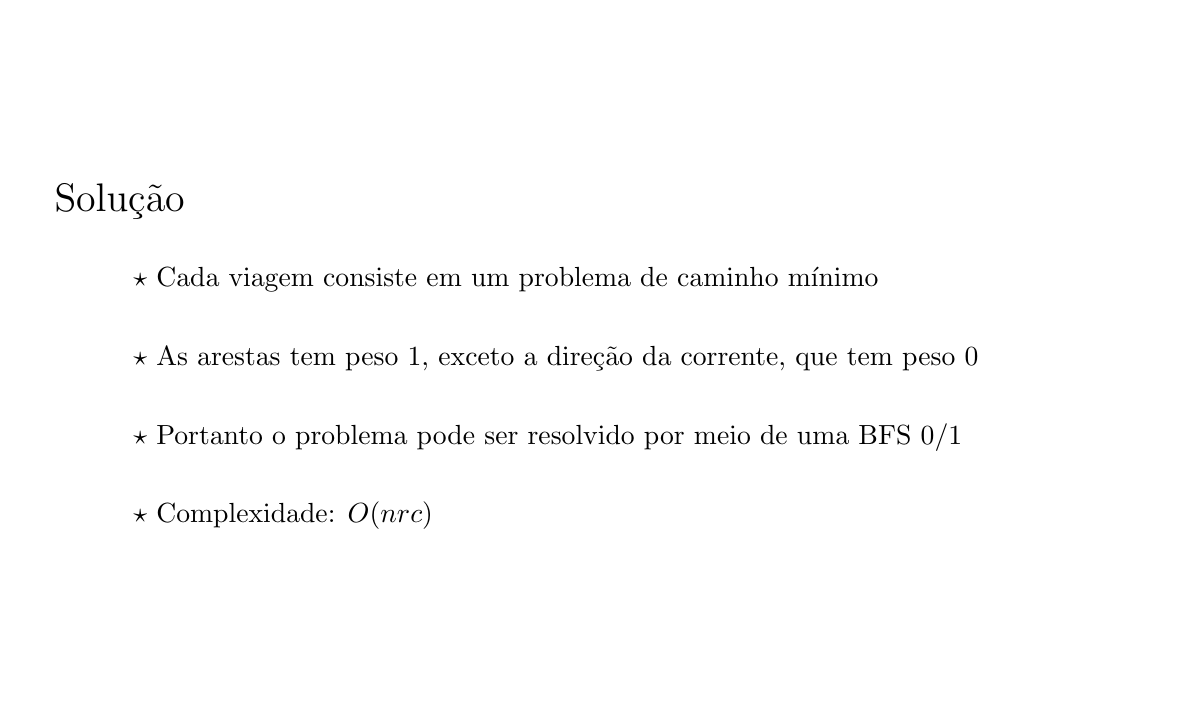
\begin{tikzpicture}
\node[draw,opacity=0] at (0, 0) {x};
\node[draw,opacity=0] at (14, 8) {x};

	\node[anchor=west] (header) at (0, 6.0) { \Large \bbbold{Solução} };


	\node[anchor=west] (a) at (1.0, 5.0) { $\star$ \bbtext{Cada viagem consiste em um problema de caminho mínimo} };


	\node[anchor=west] (b) at (1.0, 4.0) { $\star$ \bbtext{As arestas tem peso $1$, exceto a direção da corrente, que tem peso $0$} };


	\node[anchor=west] (c) at (1.0, 3.0) { $\star$ \bbtext{Portanto o problema pode ser resolvido por meio de uma BFS 0/1} };


	\node[anchor=west] (d) at (1.0, 2.0) { $\star$ \bbbold{Complexidade:} $O(nrc)$ };

\end{tikzpicture}
\end{frame}
\begin{frame}[plain,t]

\inputsnippet{cpp}{10}{29}{codes/11573.cpp}

\end{frame}
\begin{frame}[plain,t]

\inputsnippet{cpp}{31}{50}{codes/11573.cpp}

\end{frame}
\end{document}
